%************************************************
\chapter{`Bird Watching'}
%************************************************
\begin{flushright}
January-April, 2013
\end{flushright}
\section{Prior Aim}
	To observe the species, time and location of birds for the period of January-April, 2013; with sufficiently spread observations in accordance with the time of the day and the day of the week, for all weeks.
% \section{Aim}
% 	To investigate if the following
% 	\begin{enumerate}
% 		\item Seasonal, viz. `Time of the year' based variation of frequency of a given species of birds (for all species)
% 		\item `Time of the day' based variation of frequency of a given species of birds
% 		\item Geography based variation of frequency of a given species of birds
% 	\end{enumerate}

\section{Observations}
	The data collected was enormous and has been made publicly available at the following link:
	\par
	\small{\url{https://docs.google.com/spreadsheet/ccc?key=0AptbewObyE3xdDJnMUVyNU1UYkhNWG91WGx3UTMwTFE#gid=0}}
	\par
	The sailient observations have been given in \autoref{birdfinal} and further details are given in \autoref{BirdObservations}.

	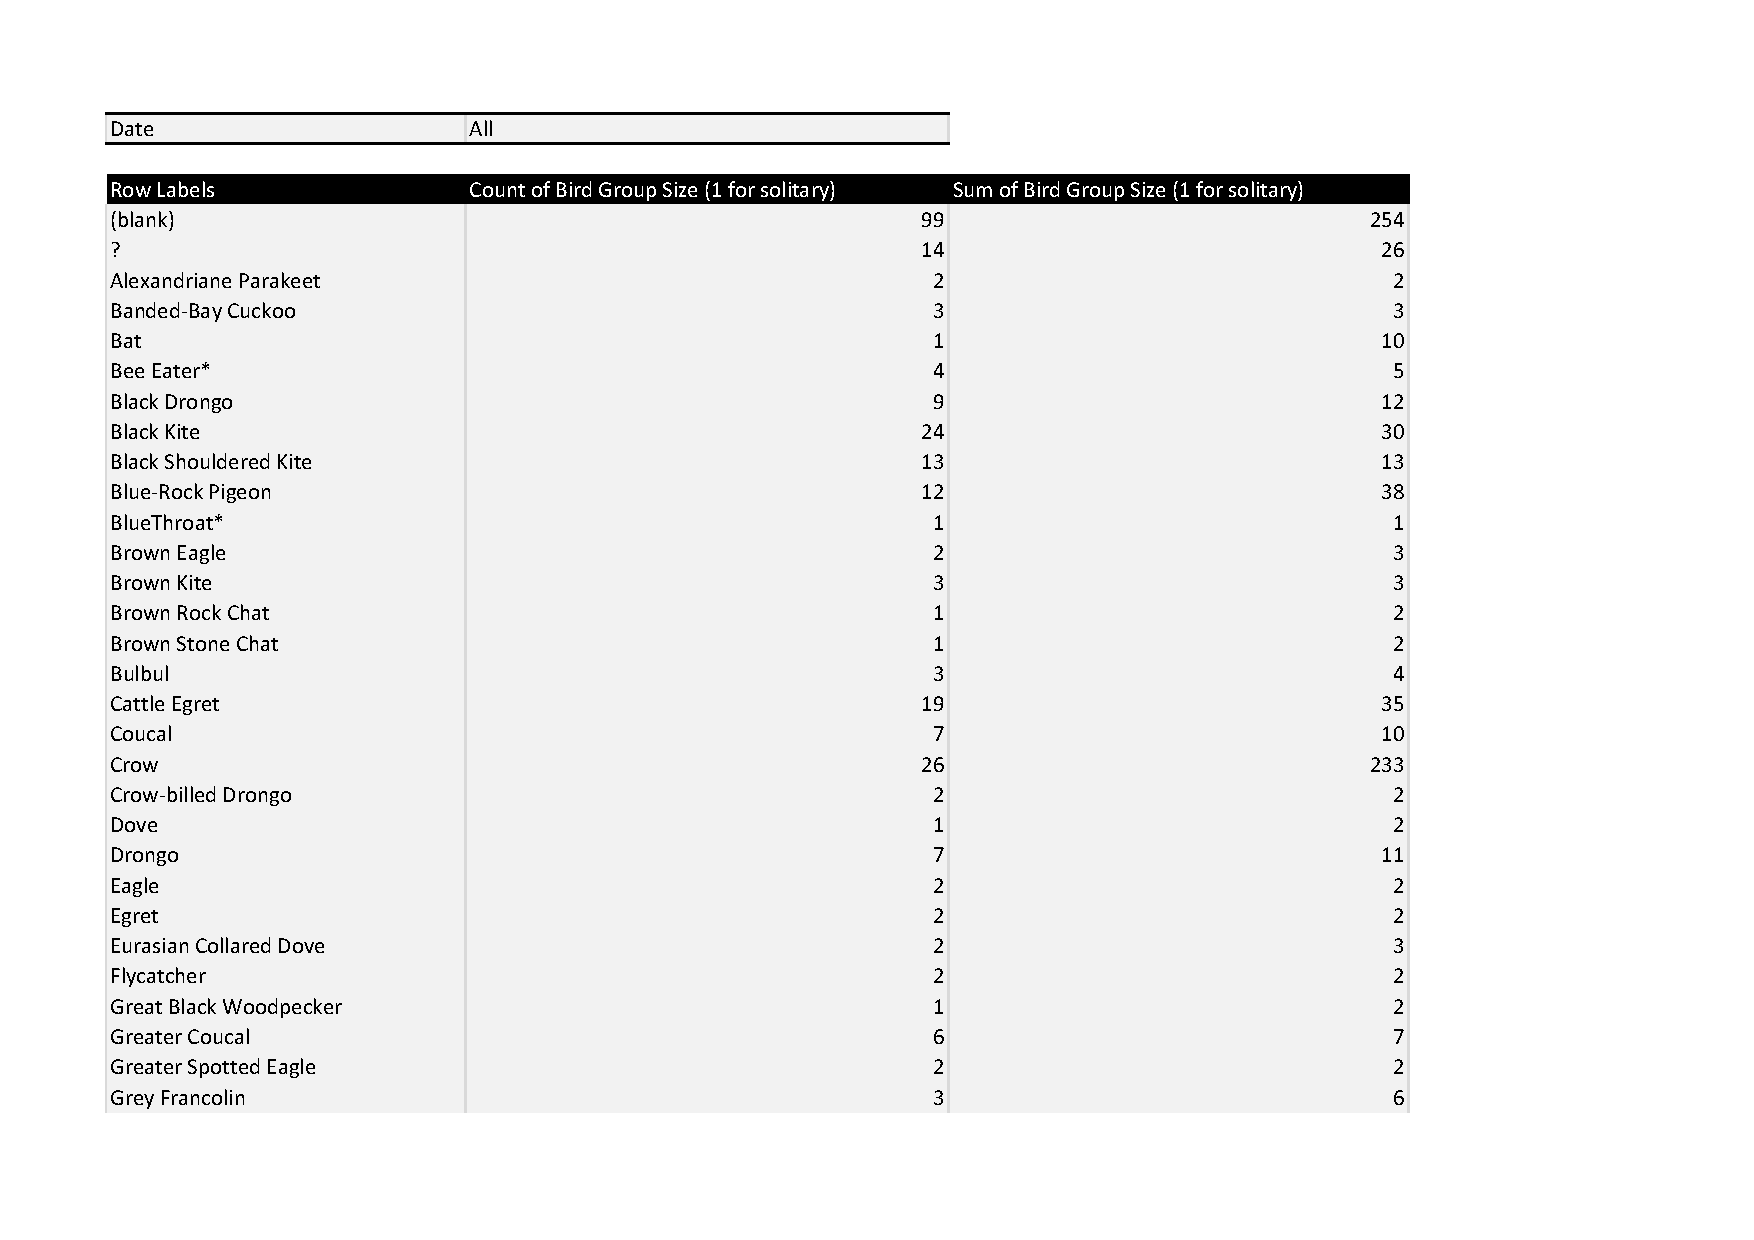
\includepdf[pages=1-,addtolist={1,table,{Bird Observations},birdfinal},pagecommand={\pagestyle{empty} \autoref{birdfinal}}]{gfx/birdy/birdy_final.pdf}

\section{Acknowledgements}
	For this experiment, in addition to our existing team, we had Yosman Bapat-dhar, Vivek Sagar, and S. Shwetha pool in their observations to form a large enough data bank. Everyone's dedicated effort has been the heart to this experiment's success.